\documentclass[11pt]{model1}

% packages
\usepackage[dvips]{graphicx}
\usepackage[french]{babel}
\usepackage[T1]{fontenc}
\usepackage{amsmath,amssymb,bbm} % math, mathbb, mathbbm

\usepackage{url} %% pour citer les url par \url
\usepackage{natbib} %% pour plus de flexibilit� dans les citations
\usepackage{makeidx} %% index
\usepackage{rotating} %% pour rotate
\usepackage{multirow} %% pour regrouper un texte sur plusieurs lignes dans une table\usepackage{multirow}
\usepackage{color} 

%\usepackage{moreverb} %% pour le verbatim en boite
%\usepackage{slashbox} %% pour couper les colonnes des tableaux en diagonale 
%\usepackage{showkeys} %% pour voir les labels
%\usepackage[all]{xy} %% pour la barre au dessus des symboles
%\usepackage{shorttoc} %% pour plusieurs tables des mati�res par la commande \shorttableofcontents{Titre}{profondeur}.
%\usepackage{textcomp} %% pour le symbol pour mille par \textperthousand.
%\usepackage[dvips]{hyperref} % permet d'obtenir des liens sur les sections dans les PDF
%\usepackage[right]{eurosym}
%\usepackage{eurosans} %% pour le symbole \euro
%\usepackage{epic,eepic}
%\usepackage{times,palatino}  % fontes
%\usepackage{mathptm}
%\usepackage{comment} % pour cut

\headheight = 13.6pt

% macros, d�finitions et nouvelles commandes perso
\def\argmax{\operatornamewithlimits{arg\,max}}
\def\argmin{\operatornamewithlimits{arg\,min}}
\newcommand{\dtc}{\ensuremath{\operatorname{d_{tc}}}}

\DeclareMathOperator*{\Mult}{Mult}

 
\makeindex 
\graphicspath{{fig/}} 


\begin{document}
\thispagestyle{empty}
\begin{titlepage}
%\TitlePageDimension

\begin{sffamily}
\begin{bfseries}

\begin{empty}
 \vspace*{58mm}
\end{empty}

\begin{flushleft}
  \hspace{60mm}
  \noindent{\Large Reuven BENICHOU}
\end{flushleft}

\begin{flushleft}
  \hspace{60mm}
  \noindent{\Large Edern HOTTE}
\end{flushleft}

\begin{flushleft}
  \hspace{60mm}
  \noindent{\Large Flavien MOULLEC}
\end{flushleft}

\vspace*{6mm}

\hspace{55mm}
\begin{minipage}[c]{0mm}
  
\includegraphics[width=110mm]{font.eps}
\end{minipage}
  
\vspace*{5mm}

\begin{flushleft}
  \hspace{46mm}
  \noindent{\huge Optimisation de biblioth�que \hspace*{46mm} de calcul num�rique}
\end{flushleft}


  \hspace{55mm}
  \noindent{\large Rapport technique du projet 11 - version 2}

  \hspace{55mm}
  \noindent{\normalsize Date : 15 Juin 2011}



  \hspace{55mm}
  \noindent{\normalsize Encadrant : Serge GUELTON}
  \newline

  \hspace{55mm}
  \noindent{\normalsize Projet de d�veloppement - Semestre 2}



  \hspace{55mm}
  \noindent{\normalsize Ann�e scolaire 2010 - 2011}
  
  \hspace{55mm}
  \noindent{\small \`A destination du groupe de pilotage du projet S2}

\end{bfseries}
\end{sffamily}

\vspace*{11mm}
\hspace{60mm}
\begin{minipage}[c]{0mm}
  \includegraphics[width=28mm]{logo.eps}
\end{minipage}
%\ResetDefaultPageDimension
\end{titlepage}

\newpage
\thispagestyle{empty}
~

%\maketitle
\newpage\cleardoublepage

\markboth{}{}
%\pagestyle{empty}
%---------------------------%
\section*{R�sum�}

Ecrire le r�sum� ici

\section*{Abstract}

Ecrire la m�me chose en Anglais

\section*{Mot-cl�s}

5-6 max

\newpage\cleardoublepage\thispagestyle{empty}
\markboth{Table des mati�res}{Table des mati�res}
\tableofcontents

\chapter{Introduction}
\label{chap:introduction}

\section{Motivations }

Le projet 11 \citep{projet11}, intitul\'e << Optimisation de biblioth\`eque de calcul num\'erique >>, est un projet informatique bas\'e sur le langage C qui vise \`a am\'eliorer 
les performances de calcul de la biblioth\`eque num-utils \citep{numutils}, travaillant sur des flots de donn\'ees \citep{dataflux}.
Il aboutira au d\'eveloppement d'un vrai logiciel qui sera publi\'e dans les archives Debian \citep{debian}.

Ceci est \'evidemment une source de motivation non n\'egligeable. Mais \`a travers cet aspect concret de notre projet, c'est tout l'environnement d'un 
projet informatique, les contraintes impos\'ees , l'interface existante entre les d\'eveloppeurs, le travail d'optimisation, qui sont les raisons 
d'\^etre de ce travail.
Il s'inscrit alors dans un contexte pr\'ecis : le d\'eveloppement d'un projet informatique en vue de sa publication.

\section{Objectifs}

Bien que le projet repose sur une optimisation de performances, l'objectif principal reste la mise en place des outils n\'ecessaires en vue de la 
r\'ealisation et de la publication d'un logiciel dans les archives Debian.  

En effet derri\`ere la probl\'ematique d'optimisation se cache une autre probl\'ematique qui sera le point de d\'epart de notre projet : comment mettre
 en \oe{}uvre un projet informatique ? 
Notre d\'emarche consistera en premier lieu en la d\'ecouverte et l'utilisation des outils n\'ecessaires \`a la r\'ealisation d'un projet informatique afin 
de mettre en ligne une biblioth\`eque num-utils cod\'e en C.
\newline 	
Tout d'abord une impl\'ementation des algorithmes sera fournie en langage C avec l'ensemble des outils de d\'eveloppement mis en \oe{}uvre. Ensuite, 
un paquet Debian fournissant une distribution open source sera mise en ligne. 
Outre les d\'ecouvertes techniques, cette premi\`ere approche sera l'occasion de constater toute l'importance de la forme ( page de manuel, readme,...) 
lors de la conception d'un logiciel informatique publi\'e.

La seconde \'etape du projet sera l'optimisation des performances de calculs de nos codes C . Cette phase, plus courte, se veut diff\'erente de la 
premi\`ere : elle n\'ecessite avant tout un travail de r\'eflexion. C'est  un travail de fond o\`u l'objectif principal sera une division par 10 du temps
 d'ex\'ecution. 

Notre d\'emarche sera donc constitu\'ee de deux \'etapes : la mise en place d'un socle de travail, puis le travail de fond d'optimisation. Ces deux phases 
s'inscrivent dans le contexte du projet qui est le d\'eveloppement d'un projet informatique afin de r\'epondre \`a la probl\'ematique explicite du sujet 
qui est l'optimisation d'une biblioth\`eque de calcul num\'erique.


 % chapitre 1

% ajouter des chapitres ici

\addcontentsline{toc}{chapter}{Conclusion}
\chapter*{Conclusion}

Au cours de notre projet, nous avons appris \`a suivre une d\'emarche de conception sp\'ecifique en vue d'aboutir \`a la cr\'eation
puis \`a la publication d'un paquet Debian. Notre travail se basait sur une biblioth\`eque de calcul num\'erique existante et d\'ej\`a
distribu\'ee num-utils. Nous avons pu montrer notre capacit\'e \`a analyser un code \'ecrit par un autre d\'eveloppeur, puis \`a l'optimiser dans 
un autre langage, en C, pr\'esentant des avantages mais \'egalement des inconv\'enients. Nous avons appris, progressivement, \`a utiliser des outils
de d\'eveloppement : le gestionnaire de version, la cr\'eation de pages de manuel (man pages), les autotools puis les outils de cr\'eation de paquets Debian. Finalement, nous obtenons une premi\`ere
version de la biblioth\`eque num-utils-ng.
\newline
\newline
Maintenant, nous devons continuer \`a am\'eliorer notre biblioth\`eque num\'erique. Il nous faut ajouter de nouvelles fonctionnalit\'es utiles et \'egalement 
corriger les bugs qui subsistent encore dans la premi\`ere version de notre biblioth\`eque num\'erique. Il nous faut aussi optimiser certains des 
algorithmes impl\'ement\'es, qui quelquefois sont un plus lents ou utilisent plus de m\'emoire que la version d\'ej\`a publi\'ee. Enfin il nous restera \`a
diffuser notre paquet. Nous avons cr\'e\'e un site internet (en construction actuellement) pour nous permettre de proposer notre distribution open source,
d'offrir une assistance technique aux futurs utilisateurs et de r\'epondre \`a leurs suggestions
\newline
\newline
L'objectif final \'etant ainsi la publication, dans les vraies archives Debian, du paquet num-utils-ng.

\markboth{Conclusion}{Conclusion}


\newpage\cleardoublepage
\bibliographystyle{abbrvnat}\bibliography{bib/references}
\addcontentsline{toc}{chapter}{References}

\newpage\cleardoublepage\addcontentsline{toc}{chapter}{Glossaire}
\chapter*{Glossaire}
\begin{description}

\item[Allocation] : l'alloction est l'op�ration qui consiste � r�server de la place dans la m�moire, c'est une op�ration qui demande un peu de ressources et qui est donc � utiliser le moins possible.
\item[autotools] : outils fournis par le projet GNU pour faciliter la fabrication de paquets � partir du code source d'un programme.
\item[Distribution] : Une distribution de GNU/Linux est une version d'un syst�me d'exploitation, il y en a plusieurs car il y a plusieurs syst�mes d'exploitation utilisant le m�me noyau : Ubuntu, Debian, Red Hat.
\item[Flux ou Flot de donn�es] : le flot de donn�es est la succession de donn�es d'un certain type, qui peuvent se poursuivre pendant un temps ind�fini.
\item [fuite de m�moire] : occupation croissante et non contr�l�e ou non d�sir�e de la m�moire d'un ordinateur. 
\item[Gestionnaire de version] : logiciel qui permet de stocker un ensemble de fichiers en conservant la chronologie de toutes les modifications qui ont �t� effectu�es dessus.
\item[Langage compil�] : langage dans lequel le code est traduit en langage binaire pour une compr�hension direct du processeur. Un programme �crit en langage compil� est traduit en instructions lisibles par la machine et peut �tre ex�cut� ind�pendamment de tout autre programme.
\item[Langage interpr�t�] : langage dans lequel le code n'est pas compil� . Un programme �crit en langage interpr�t� n'est pas ex�cut� directement par la machine mais par un autre programme.
\item[logiciel open source] : logiciel dont l'utilisation, l'�tude, la modification et la duplication en vue de sa diffusion sont permises, techniquement et l�galement.
\item[Makefile] : un Makefile est un fichier utilis� par la commande make des distributions GNU/Linux permettant l'automatisation de t�ches simples telles que la compilation.
\item[mode] : le mode d'une s�rie de nombres est le nombre qui apparait le plus de fois dans la s�rie.
\item[Paquet] : un paquet Debian est un paquet rassemblant les sources d'un programme et comment les installer, ainsi que les d�pendances n�cessaires. On les trouve typiquement dans les archives Debian et elle servent � installer des programmes facilement sous Ubuntu ou Debian.

\end{description}

\markboth{Glossaire}{Glossaire}

\appendix
\chapter{R\'epartition de la r\'edaction et de la relecture du rapport}

Voici la r\'epartition de l'\'ecriture et de la relecture du rapport :
\newline
\section{\'Ecriture}
\begin{itemize}
  \item[-] R\'esum\'e/Abstract : Edern
  \item[-] Chapitre 1 : \textbf{Introduction} : Reuven
  \item[-] Chapitre 2 : \textbf{La Biblioth\`eque num-utils} : Flavien
  \item[-] Chapitre 3 : \textbf{D\'emarche de conception effectu\'e}, section 1 : Reuven
  \item[-] Chapitre 3 : \textbf{D\'emarche de conception effectu\'e}, section 2 et 3 : Flavien
  \item[-] Chapitre 4 : \textbf{Tests et Optimisation} : Edern
  \item[-] Conclusion : Flavien
\newline
\end{itemize}
\section{Relecture}
\begin{itemize}
  \item[-] R\'esum\'e/Abstract : Reuven
  \item[-] Chapitre 1 : \textbf{Introduction} : Flavien
  \item[-] Chapitre 2 : \textbf{La Biblioth\`eque num-utils} : Edern
  \item[-] Chapitre 3 : \textbf{D\'emarche de conception effectu\'e} : Edern
  \item[-] Chapitre 4 : \textbf{Tests et Optimisation} : Flavien
  \item[-] Conclusion : Edern
\end{itemize}


\newpage
\cleardoublepage
\addcontentsline{toc}{chapter}{Index}
\markboth{Index}{Index}
\printindex

\newpage\thispagestyle{empty}   % affiche la derni�re page du rapport
\vspace*{55mm}
\hspace{48mm}
\begin{minipage}[c]{0mm}
  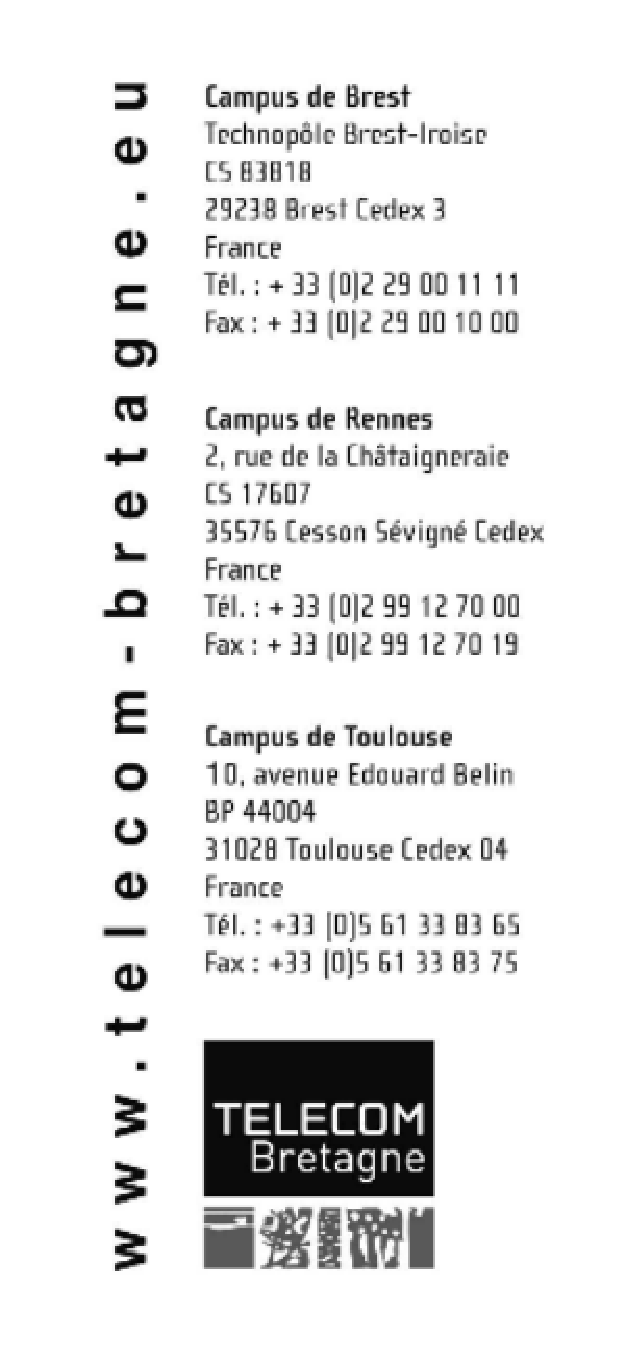
\includegraphics[width=55mm]{lastPage.eps}
\end{minipage}

\end{document}
